\chapter{Introduction}
\label{introduction}
Route information and navigation guidance provided by modern navigation applications can be redesigned to motivate drivers to choose unselfish routes. Doing so will realize their potential in managing traffic flow, adding positive social value for daily commuters. In 2050, we will see almost 70\% of the global population move to cities, increasing car ownership and potentially affecting our goals of achieving sustainability. These additional vehicles will slowly congest denser urban environments and complex road networks, worsening traffic conditions and bring forth a number of negative consequences \cite{Mehndiratta2017}. While our current road networks and transportation systems are still keeping up with the rising demand, modern navigation applications such as Waze and Google Maps, and in-car navigation systems found in modern car models today are offering a slight reprieve in dealing with daily traffic conditions. At their core, these tools provide digital maps that show route options, traffic conditions, and other road or traffic advisories. To reduce driving distraction, they also give turn-by-turn directions towards a destination. As commercial products, we are provided with a diverse array options which we can compare in terms of mobility, frequency of map updates and available information (Figure \ref{fig:navi-tools-spectrum}). 

\begin{figure}[t]
  \centering
  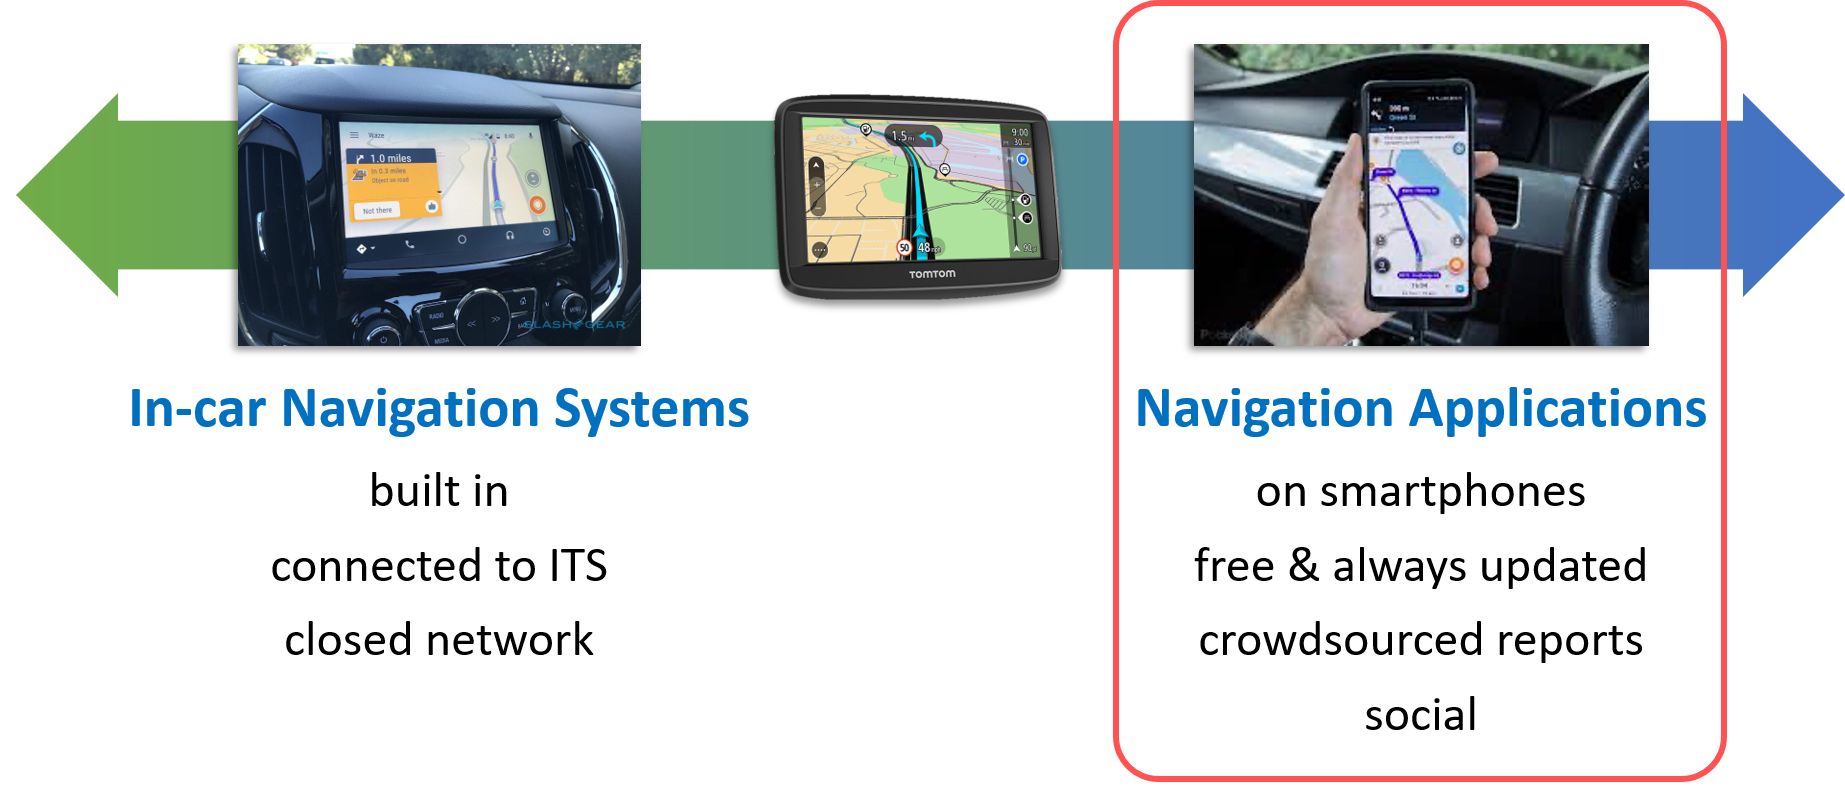
\includegraphics[scale=0.45]{figures/navi-tools-spectrum.png}
  \caption{The spectrum of navigation tools that are available commercially for drivers. Leftmost are in-car navigation systems which typically come with a vehicle. Such navigation tools are different per car make and model. One of their main advantages is that they can communicate with other cars of the same car make and access to maps do not need connection to the Internet. In the middle are satellite navigation tools or GPS devices. These can be bought separately from navigation companies (e.g. Tomtom and Garmin) and can be mounted on any car. Rightmost are modern navigation applications like Google Maps and Waze. They are run on smartphones and access to the most recent maps and route information is mostly free.}
  \label{fig:navi-tools-spectrum}
\end{figure}

In this dissertation, I focus my investigation and designs for navigation applications, as they democratize the access to navigation services. As their core routing service becomes more advanced with machine learning and sensing capabilities, navigation applications are becoming integral in many commutes to monitor regular routes, to discover new ones and sometimes to avoid traffic congestion. These modern tools are free to download on most smartphones, have the latest maps, and with some utilizing the Intelligent Transportation Systems of advanced cities. Maximizing built-in sensors and modern GPS, they collect floating car data to learn traffic conditions and further augments these with crowd-sourced reports from ordinary users \cite{Levine2014SystemExchange, Valdes-Dapena2016MostDirections}. All these information are fed into machine learning algorithms to produce models that can power their sophisticated routing algorithms, allowing drivers to cut through traffic by sometimes suggesting unfamiliar routes and small, residential roads. 

\section{Negative Externalities}
Since the first GPS devices were made commercially available to consumers, engineers and designers have always centered their features around the individual driver. Understandably, this has resulted to their modern commercial success as most modern car models include in-car navigation systems by default. For those who do not have that luxury, they can still download free navigation applications like Google Maps and Waze, which also offer turn-by-turn voice guidance. 

A large user base has been a benchmark for an application's success. However, the widespread use of such applications can sometimes have negative externalities as shown by a recent work of Bayen et. al. In an agent-based model simulation, they have shown that as more drivers follow the shortcuts provided by navigation applications, smaller residential roads that run parallel or connected to highways experience unlikely congestion. Unlike traffic congestion on highways which can dissipate fast, these small roads will experience congestion for longer because of their low carrying capacity\cite{Thai2016NegativeApproach}. Insights from this model are also supported by anecdotal evidence of cities like Los Angeles experiencing local unprecedented disruptions because of drivers using Waze \cite{Battelle2016TheShift, Thornton2015HowTimes, Wirtschafter2017DrivingKALW}. These unexpected negative effects have prompted some local communities to start gaming the system \cite{Weise2017WazeAlgorithms} and some government officials to take legal action \cite{Farivar2018LATechnica}. I argue that the major reason for this is how designers of navigation applications continue to only follow the principle that drivers want the fastest or shortest path to their destinations (selfish Wadrop equilibrium\cite{wardrop1952road}). Instead of directly addressing the problem of traffic congestion, these applications provide shortcut routes, promoting individualistic choices at the expense of other stakeholders in the system (e.g. other drivers, households in residential roads). Inadvertently, they cause transportation networks to fall into inefficiency, showing the price of anarchy\cite{wardrop1952road}. 

As beneficial as these navigation applications can be for individual drivers to avoid traffic congestion or get to their destinations faster, it is worth looking into how we can include other stakeholders into the design of such applications and their algorithms to safeguard the interest of the communities where they operate. At the same time, we should investigate how navigation applications can reduce individualistic choices in other trip contexts. 

\section{Imagining a Distributed Future}
Because of their fast technological advancements and ubiquity, many government stakeholders are optimistic of the potential of navigation applications in shaping sustainable driving behaviors \cite{Attard2016TheSystems}. Here, I envision a future in which governments can manage traffic flow on their roads by recommending unselfish routes to drivers. Following Wardrop's second principle\cite{wardrop1952road}, consider the toy problem shown in Figure \ref{fig:system-optimal}. In a \textit{user equilibrium} scenario in which each driver chooses their own fastest route and ends up using all possible paths, many of them will include road \textit{BC} in their routes because it has a small link cost or fast travel time. Eventually, everyone's average travel time becomes 3.75 minutes. Now let’s say cars are centrally distributed in the road network. So instead of letting them use all possible roads, it now distributes 50 cars each to use routes \textit{ABD} and \textit{ACD}. Since nobody is taking the shortcut path anymore (road \textit{BC}), everyone’s average travel time becomes faster, from 3.75 minutes to 3.5 minutes. If we could rethink current features and designs of navigation applications to start encouraging unselfish routes that can lead to more sustainable futures, I believe that navigation applications has the potential for more. Implementing this in free applications can have a great impact because there is higher chance of mass adoption. But realizing this vision will take a concerted effort to address different aspects of the solution. In terms of the underlying infrastructure and sensing capabilities, there are still many open challenges on data sparsity and in ensuring the integrity of crowd-sourced reports \cite{Silva2016UsersOpportunities,QingYang2015TowardNetworks,Vyroubal2016MobileSystems}. However in this dissertation, I focus on the human-computer interaction aspect of this problem, specifically on drivers' route choice and navigation behaviors. 

\begin{figure}[t]
  \centering
  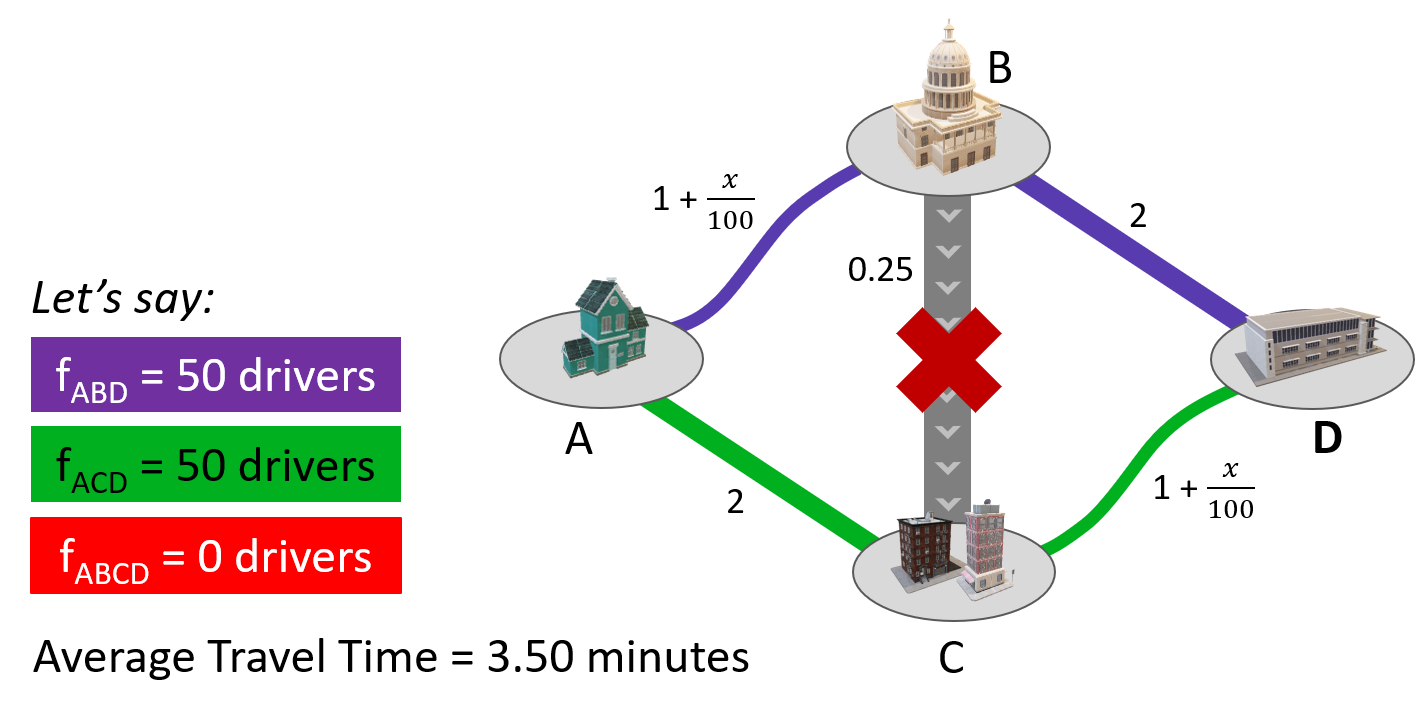
\includegraphics[scale=0.6]{figures/system-optimal.png}
  \caption{A toy problem illustrating a central distribution of drivers. This road network has 3 possible routes, with road BC as a one-way road. In a system optimal scenario, 100 drivers are equally distributed between routes \textit{ABD} and \textit{ACD}. Road \textit{BC} is unused because it significantly increases the traffic flow in roads \textit{AB} and \textit{CD}. Not using all possible routes consequently reduced the average travel time of everyone to just 3.5 minutes, from 3.75 minutes in a user equilibrium scenario. This was recreated from Figure 1 of Colak et. al.\cite{colak2016understanding}.}
  \label{fig:system-optimal}
\end{figure}

\section{Interaction with Navigation Applications Today}
In recent years, in-car navigation systems and their mobile application counterparts have gained popularity among drivers \cite{2018GoogleAnnieb, Waze2016DriverIndex}, especially those driving in cities and other urban areas with increasingly complex road networks. Looking at the user's experience, several studies have found older drivers experiencing difficulties following the voice navigation \cite{Dingus1997a,Mahmud2009UserDrivers} while younger drivers overly rely on the turn-by-turn navigation \cite{Mahmud2009UserDrivers}. More recently, Brown \& Laurier enumerated five \emph{normal, natural troubles} of driving with GPS devices with regards to defining destinations, quality of routes, accuracy of maps and sensors, timing and relevance of instructions, and legality of recommendations \cite{Brown2012TheGPS}. All these have profound effects on achieving a positive experience.

By default, drivers are recommended the fastest route to their destinations, with alternative routes either shown up front (i.e. Google Maps) or hidden for you to discover (i.e. Waze). While many people agree and say that they do want fast or short routes when asked at any given day, asking them again in actual driving contexts shows otherwise \cite{Pfleging2014ExperienceNavigation}. This is further supported by empirical evidence from GPS tracks and recorded actual trips that show drivers' repeated non-preference of recommended fastest routes \cite{Quercia2014, Zhu2015DoPrinciple,Tang2016AnalyzingData} and sudden deviations\cite{Fujino2018DetectingTracks,Brown2012TheGPS,Samson:2019:EFI:3290605.3300601}. While there is great support for drivers to make decisions before starting a trip, there are gaps in current systems and applications that fail to consider their changing needs, contexts and preferences, which ultimately affect their compliance on the recommendation.

In Brown \& Laurier's work\cite{Brown2012TheGPS}, after they describe the common dilemmas faced by drivers and passengers with traditional GPS devices, they argued that in order for drivers to have more positive experiences and better \textit{instructed actions}, developers should focus more on supporting their interpretation and analysis of new route guidance and information. Instead of assuming that drivers have zero knowledge, navigation applications should allow them figure out what to do next.

Looking at these challenges and how we want future navigation applications to become tools in encouraging sustainable driving behaviors, I focus my line of research on answering this central research question: \textbf{\textit{How can we encourage drivers to follow unselfish routes in their daily commutes?}} Specifically, I see two main challenges that needed to be addressed:
\begin{itemize}
    \item How do we encourage drivers to choose unselfish routes before a trip?
    \item How do we make sure that drivers continue to follow an unselfish route (if they choose to do so) or convince them to switch to an unselfish route in the middle of a trip?
\end{itemize}

Additionally, how do we achieve these while supporting their sense of agency in their navigation decisions?

\section{Encouraging Unselfish Routes}
In order to redesign route information and navigation guidance provided by modern navigation applications to motivate drivers to choose unselfish routes, I started with a formative study that deepened my understanding of a driver’s use of navigation applications. Using key insights and design implications, I refined my research questions and began the process of rethinking navigation applications as a form of civic technology by evaluating two separate approaches -- each focused on a different phase of the driving navigation task. I cap-off my PhD research by combining the two approaches and refining their designs to form a holistic approach towards a personality-targeted navigation application. After reading this dissertation, I hope I can convince you that navigation applications can be more than a routing tool and can be transformed into a civic technology for social good. Figure \ref{fig:overview} shows the different studies I conducted to answer my central research question.

\begin{figure}[t]
  \centering
  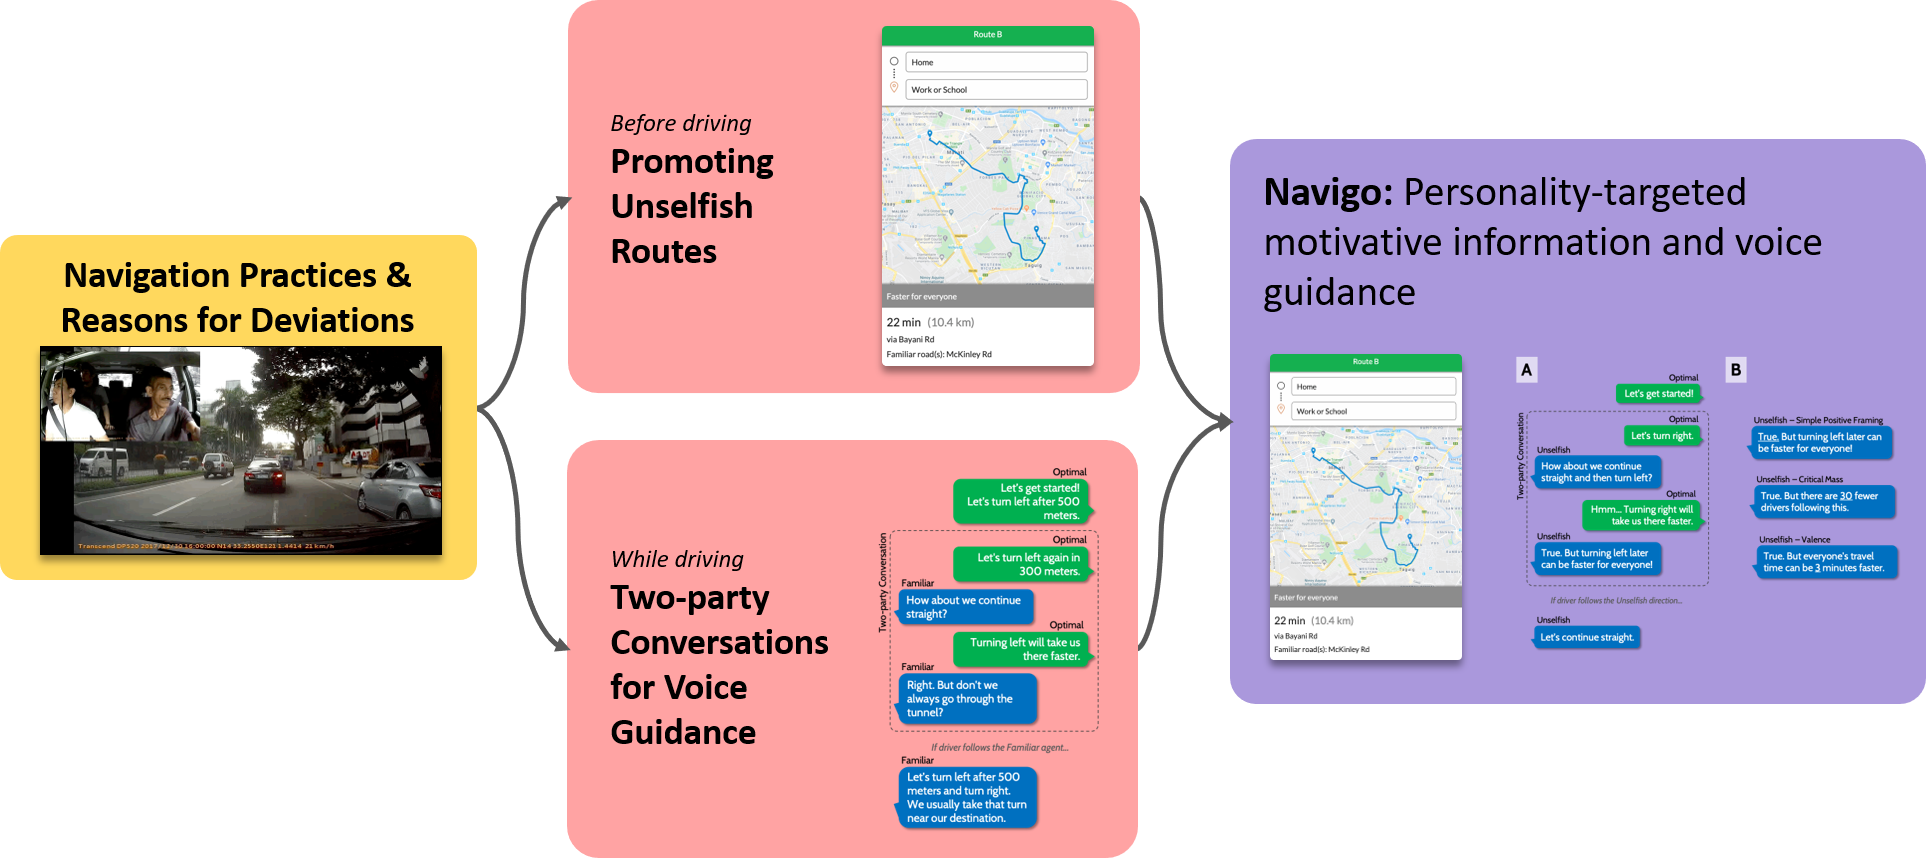
\includegraphics[scale=0.4]{figures/overview.png}
  \caption{Overview of the different studies I conducted over the course of three years as I gained a deeper understanding of driver experiences with modern navigation applications and explored different motivational techniques for displaying route information and delivering navigation guidance.}
  \label{fig:overview}
\end{figure}

\section{Structure}
I begin this dissertation by reviewing the previous literature around navigation applications, HCI of recommender systems, traffic psychology and behavior, and factors that affect route choice (Chapter \ref{ChapterRL}). In Chapter \ref{ChapterInteractNavi}, I describe a formative study that investigates how drivers interact with modern navigation applications and what affects their route choices. In order to support the self-efficacy and agency of drivers, Chapter \ref{ChapterSDT} discusses Self-Determination Theory which focuses on the different types of motivation and what techniques can be used to internalize motivation. It is then used to inform the designs in this dissertation. In Chapter \ref{ChapterPreTrip}, we explore the use of the Self-Determination Theory in designing autonomy-supportive navigation applications and investigate the effects of adding motivative and familiarity information to encourage the choice unselfish routes before a trip. In Chapter \ref{ChapterConversations}, I focus on the on-trip voice guidance and explore the use of two-way conversations to influence route choice when an alternative route is made available. Then in Chapter \ref{ChapterNavigo}, I integrate the display of pre-trip motivative and familiarity information with the delivery of two-party conversations as voice guidance. I conclude this dissertation with a summary of my key contributions as well as an envisioning of future directions towards the design and evaluation of altruistic navigation applications (Chapter 8).
